% =========================================================================
% IEEE Transactions / Conference Paper
% Title: Dense Wavelength Division Multiplexing Using Thermally Tunable
%        Racetrack Microring Resonators on Silicon-on-Insulator
% Template: IEEEtran class (journal mode)
% =========================================================================
\documentclass[journal]{IEEEtran}

% --- Packages ---------------------------------------------------------------
\usepackage[T1]{fontenc}
\usepackage[utf8]{inputenc}
\usepackage{amsmath,amssymb,amsfonts}
\usepackage{algorithmic}
\usepackage{graphicx}
\usepackage{textcomp}
\usepackage{xcolor}
\usepackage{booktabs}
\usepackage{siunitx}
\usepackage{hyperref}
\usepackage{cite}
\usepackage{float}

% SI unit configuration
\sisetup{per-mode=symbol, detect-all}

% Hyperref configuration
\hypersetup{
    colorlinks=true,
    linkcolor=blue,
    citecolor=blue,
    urlcolor=blue,
    pdftitle={DWDM Using Thermally Tunable Racetrack Microring Resonators},
    pdfauthor={Author Names}
}

% ============================================================================
\begin{document}

\title{Dense Wavelength Division Multiplexing Using Thermally Tunable\\
       Racetrack Microring Resonators on Silicon-on-Insulator}

\author{First~Author,~\IEEEmembership{Student Member,~IEEE,}
        Second~Author,~\IEEEmembership{Member,~IEEE,}
        and~Third~Author,~\IEEEmembership{Senior Member,~IEEE}%
\thanks{This work was supported in part by [Funding Agency].}%
\thanks{The authors are with the Department of Electronics and Communication
Engineering, [Institution Name], [City], [Country] (e-mail:
first.author@institution.edu).}%
\thanks{Manuscript received \today; revised [Date].}}

% --- Abstract ---------------------------------------------------------------
\markboth{IEEE Transactions on Photonics,~Vol.~X, No.~X, \MakeUppercase{Month}~20XX}%
{Author \MakeLowercase{\textit{et al.}}: DWDM Using Thermally Tunable Racetrack MRRs}

\maketitle

\begin{abstract}
We present the design, simulation, and analysis of a dense wavelength
division multiplexing (DWDM) demultiplexer based on thermally tunable
racetrack microring resonators (MRRs) fabricated on a silicon-on-insulator
(SOI) platform. The device employs titanium nitride (TiN) microheaters
integrated directly above the waveguide straight-coupling sections to
achieve wavelength tuning with low power consumption. Each racetrack
resonator is designed to address one International Telecommunication Union
(ITU) channel in the C-band (\SIrange{1530}{1565}{\nano\meter}) on a
\SI{100}{\giga\hertz} grid. Parametric gdsfactory design scripts automate
the generation of GDSII mask layouts for arbitrary channel counts. Full
electromagnetic simulations using the MEEP (MIT Electromagnetic Equation
Propagation) FDTD engine verify the spectral response, yielding an
extinction ratio (ER) exceeding \SI{20}{\decibel}, insertion loss (IL)
below \SI{0.25}{\decibel}, and a quality factor $Q > 9{,}600$ for all
channels. Thermal tuning efficiency is characterised at
\SI{688}{\pico\meter\per\milli\watt}, enabling re-alignment to any ITU
channel within a \SI{\pm 2}{\nano\meter} window at under \SI{3}{\milli\watt}
per channel. The design is fully
process-compatible with standard \SI{220}{\nano\meter} SOI multi-project
wafer (MPW) runs and the results are directly reproducible from the
open-source scripts provided.
\end{abstract}

\begin{IEEEkeywords}
Racetrack microring resonator, silicon photonics, DWDM, wavelength division
multiplexing, thermal tuning, TiN microheater, MEEP, FDTD, gdsfactory,
silicon-on-insulator.
\end{IEEEkeywords}

% ============================================================================
\section{Introduction}
\label{sec:intro}
Silicon photonics has emerged as a leading platform for large-scale
photonic integration owing to its compatibility with complementary
metal-oxide-semiconductor (CMOS) fabrication infrastructure, high
index contrast, and the availability of multi-project wafer (MPW)
services~\cite{reed2010silicon, bogaerts2012silicon}.  Among the
building blocks of silicon photonic integrated circuits (PICs), microring
resonators (MRRs) and their elongated variants---racetrack
resonators---play a pivotal role in wavelength-selective routing,
filtering, modulation, and sensing~\cite{little1997microring,
yariv2000critical}.

Dense wavelength division multiplexing (DWDM) leverages the high
spectral efficiency of closely spaced optical channels to maximise
the information capacity of a single fibre or waveguide
bus~\cite{winzer2012optical}. In the C-band,
the International Telecommunication Union (ITU) G.694.1 standard
defines a \SI{100}{\giga\hertz} (\SI{\sim 0.8}{\nano\meter}) channel
grid, placing stringent requirements on the resonance wavelength
accuracy and thermal stability of ring-based demultiplexers.

Thermal tuning via integrated microheaters is the most widely adopted
post-fabrication technique for compensating fabrication-induced
resonance shifts and for dynamic channel
assignment~\cite{dong2010thermally, watts2013adiabatic}. Titanium
nitride (TiN) is preferred as the heater material in CMOS-compatible
flows because of its low electrical resistivity, mechanical stability,
and optical absorption properties that minimise parasitic waveguide
loss~\cite{sacher2014wide}.

Despite the broad literature on individual ring modulators and switches,
a complete open-source workflow---from parametric GDSII layout generation
through electromagnetic simulation to manuscript-ready figures---for a
multi-channel DWDM demultiplexer based on racetrack MRRs is still
lacking.  This paper addresses that gap with the following contributions:

\begin{enumerate}
  \item A parametric gdsfactory-based design script that generates
        foundry-ready GDSII layouts for a configurable number of ITU
        C-band channels (Section~\ref{sec:layout}).
  \item Full-wave FDTD simulation using MEEP of the through- and
        drop-port spectral responses, including temperature-dependent
        refractive index shifts (Section~\ref{sec:simulation}).
  \item Systematic extraction of key performance metrics: extinction
        ratio (ER), insertion loss (IL), quality factor $Q$, free
        spectral range (FSR), and inter-channel crosstalk
        (Section~\ref{sec:results}).
  \item Characterisation of the thermal tuning efficiency and power
        budget for a \SI{\pm 2}{\nano\meter} tuning range
        (Section~\ref{sec:thermal}).
\end{enumerate}

The remainder of the paper is organised as follows.
Section~\ref{sec:design} introduces the device architecture and
physical parameters.  Section~\ref{sec:layout} describes the automated
layout generation flow.  Sections~\ref{sec:simulation}--\ref{sec:thermal}
present the simulation methodology and results.
Section~\ref{sec:conclusion} concludes the paper.


% ============================================================================
\section{Device Architecture and Design Parameters}
\label{sec:design}
\subsection{SOI Waveguide Platform}
The device is built on the standard \SI{220}{\nano\meter}
silicon-on-insulator (SOI) platform with a \SI{2}{\micro\meter} buried
oxide (BOX) layer.  Strip waveguides with a cross-section of
\SI{500}{\nano\meter} $\times$ \SI{220}{\nano\meter} support a single
quasi-transverse-electric (TE) mode at \SI{1550}{\nano\meter} with a
simulated effective index $n_\text{eff} = 2.437$ and group index
$n_g = 4.182$.

\subsection{Racetrack Geometry}
A racetrack resonator consists of two straight coupling sections of
length $L_c$ connected by two semicircular bends of radius $R$.  The
total round-trip optical path length is
\begin{equation}
  L_\text{rt} = 2 L_c + 2\pi R.
  \label{eq:roundtrip}
\end{equation}
Resonance occurs when $L_\text{rt}$ is an integer multiple of the
effective wavelength:
\begin{equation}
  m\lambda_m = n_\text{eff}(\lambda_m)\,L_\text{rt},
  \label{eq:resonance}
\end{equation}
where $m$ is the longitudinal mode order.  Table~\ref{tab:params} lists
the nominal design parameters for the eight-channel demultiplexer.

\begin{table}[!t]
\caption{Racetrack MRR Design Parameters}
\label{tab:params}
\centering
\begin{tabular}{lSs}
\toprule
\textbf{Parameter} & \textbf{Value} & \textbf{Unit} \\
\midrule
Waveguide width $w$            & 500  & \nano\meter \\
Waveguide height $h$           & 220  & \nano\meter \\
Bend radius $R$                & 10   & \micro\meter \\
Coupling-section length $L_c$  & 15   & \micro\meter \\
Gap $g$ (bus--ring)            & 150  & \nano\meter \\
Gap $g$ (ring--drop)           & 150  & \nano\meter \\
Round-trip length $L_\text{rt}& 92.83& \micro\meter \\
FSR (at \SI{1550}{\nano\meter})& 6.19 & \nano\meter \\
TiN heater width               & 1    & \micro\meter \\
TiN heater thickness           & 100  & \nano\meter \\
Heater offset above waveguide  & 1    & \micro\meter \\
\bottomrule
\end{tabular}
\end{table}

\subsection{Coupling-Region Design}
The power coupling coefficient $\kappa^2$ is engineered via the gap $g$
and coupling length $L_c$ to achieve critical coupling at each
resonance wavelength, minimising through-port transmission to zero and
maximising drop-port power.  The coupling coefficient relates to the
transmission matrix of the directional coupler~\cite{okamoto2006fundamentals}:
\begin{equation}
  \begin{pmatrix} E_\text{out,1} \\ E_\text{out,2} \end{pmatrix}
  =
  \begin{pmatrix} t & j\kappa \\ j\kappa & t \end{pmatrix}
  \begin{pmatrix} E_\text{in,1} \\ E_\text{in,2} \end{pmatrix},
  \label{eq:coupler}
\end{equation}
where $t^2 + \kappa^2 = 1$ for a lossless coupler.

For a symmetric add-drop ring, the critical-coupling condition requires
$|t| = a^{1/2}$, where $a$ is the round-trip field amplitude transmission
(related to the propagation loss $\alpha$ by $a = e^{-\alpha L_\text{rt}/2}$).

\subsection{Channel-to-Channel Spacing}
Eight ITU C-band channels centred at \SIlist{1544.5; 1545.3; 1546.1;
1546.9; 1547.7; 1548.5; 1549.3; 1550.1}{\nano\meter}
(\SI{100}{\giga\hertz} grid) are targeted.  To fit all resonances within
one FSR, the straight-section lengths are individually adjusted by
\begin{equation}
  \Delta L_c^{(k)} = \frac{(k-1)\Delta\lambda_\text{ch}\,n_g}
                          {n_g - n_\text{eff}}\,\frac{L_\text{rt}}{2R},
  \label{eq:delta_lc}
\end{equation}
where $k \in \{1,\ldots,8\}$ is the channel index and
$\Delta\lambda_\text{ch} \approx \SI{0.8}{\nano\meter}$.


% ============================================================================
\section{Parametric Layout Generation with gdsfactory}
\label{sec:layout}
Mask layouts are generated programmatically using
\texttt{gdsfactory}~\cite{gdsfactory}, a Python library for parametric
photonic component design and GDS~II export.  All geometric parameters
(bend radius, coupling length, gap, channel count, channel spacing) are
centralised in a single configuration dictionary, enabling rapid design-space
exploration without manual editing of the GDS file.

\subsection{Component Hierarchy}
The top-level cell \texttt{dwdm\_demux} instantiates:
\begin{enumerate}
  \item An \emph{input bus waveguide} routed from the chip facet to the
        first racetrack coupling region.
  \item $N$ \emph{racetrack resonator} sub-cells, each containing the
        ring geometry, the through-/drop-port bus stubs, and the TiN
        heater metal layer.
  \item $N$ \emph{drop-port waveguides} fanning out to individual output
        facets or fibre-coupling sites.
  \item \emph{Metal routing layers} connecting the heater contacts to
        bond-pad arrays at the chip periphery.
\end{enumerate}

\subsection{Layer Stack}
The design uses four GDS layers consistent with a generic \SI{220}{\nano\meter}
SOI foundry PDK:
\begin{itemize}
  \item \texttt{WG} (layer 1): silicon strip waveguide etch.
  \item \texttt{HEATER} (layer 4): TiN heater definition.
  \item \texttt{M1} (layer 31): first metal (Al or Cu) heater contacts.
  \item \texttt{LABEL} (layer 66): text labels for port identification.
\end{itemize}

\subsection{Automated Layout Script}
Fig.~\ref{fig:layout} shows the generated GDSII layout for an 8-channel
demultiplexer.  The script \texttt{design/dwdm\_demux.py} accepts command-line
arguments for the number of channels, channel spacing, and output filename,
and can be called as:
\begin{verbatim}
python design/dwdm_demux.py \
    --channels 8 \
    --spacing_ghz 100 \
    --output dwdm_8ch.gds
\end{verbatim}

\begin{figure}[!t]
  \centering
  \includegraphics[width=\columnwidth]{figures/layout_8ch}
  \caption{Simulated GDSII layout of the 8-channel DWDM demultiplexer
           generated by the parametric gdsfactory script.  Each racetrack
           resonator is colour-coded by channel.  Metal heater contacts
           and bond pads are shown in the upper routing region.}
  \label{fig:layout}
\end{figure}


% ============================================================================
\section{Electromagnetic Simulation Methodology}
\label{sec:simulation}
Full-wave FDTD simulations are performed using MEEP
(MIT Electromagnetic Equation Propagation)~\cite{oskooi2010meep}, an
open-source C++/Python FDTD package.  The simulation workflow consists
of three stages: (i)~mode-source computation to identify the fundamental
TE mode at each frequency, (ii)~time-domain propagation to compute the
S-parameters, and (iii)~post-processing to extract the spectral response
and performance metrics.

\subsection{Simulation Domain}
A 2-D cross-sectional simulation in the $xy$-plane is used for rapid
modal analysis, while 3-D simulations of the full racetrack geometry
(with a $z$-dimension that captures the SOI slab mode profile) are used
for accurate insertion-loss prediction.  Perfectly matched layer (PML)
boundary conditions of thickness \SI{1}{\micro\meter} surround the
computational domain.

\subsection{Simulation Resolution and Materials}
A spatial resolution of \SI{20}{\nano\meter} (corresponding to
50~pixels\,/\,\SI{}{\micro\meter}) is used in 2-D and \SI{50}{\nano\meter}
in 3-D.  Material dispersions are modelled using Sellmeier fits:
\begin{itemize}
  \item \emph{Silicon}:
        $n_\text{Si}(\lambda) = \sqrt{11.97 +
        \tfrac{0.939}{\lambda^2 - 0.028}}$ (wavelength in \si{\micro\meter})
  \item \emph{SiO\textsubscript{2}}:
        $n_\text{SiO_2}(\lambda) = \sqrt{1 +
        \tfrac{0.696\lambda^2}{\lambda^2-0.0047} +
        \tfrac{0.408\lambda^2}{\lambda^2-0.013} +
        \tfrac{0.897\lambda^2}{\lambda^2-97.9}}$
\end{itemize}

\subsection{Thermal Refractive Index Model}
Temperature-dependent resonance tuning is modelled by applying a
spatially uniform perturbation $\Delta n_\text{Si}$ to the silicon
refractive index across the waveguide cross-section:
\begin{equation}
  \Delta n_\text{Si}(T) = \frac{dn}{dT}\,\Delta T,
  \quad \frac{dn}{dT}\bigg|_\text{Si} = \SI{1.84e-4}{\per\kelvin},
  \label{eq:thermo_optic}
\end{equation}
which produces a resonance shift
\begin{equation}
  \Delta\lambda_\text{res} = \frac{\lambda_\text{res}}{n_g}\,
  \Gamma\,\frac{dn}{dT}\,\Delta T,
  \label{eq:resonance_shift}
\end{equation}
where $\Gamma$ is the confinement factor of the waveguide mode in silicon.

\subsection{S-Parameter Extraction}
Flux planes are placed at the input port (port 1), through port (port 2),
and drop port (port 3).  After a normalisation run (straight waveguide),
the through-port transmission $T_\text{through} = |S_{21}|^2$ and
drop-port transmission $T_\text{drop} = |S_{31}|^2$ are computed over
the wavelength range \SIrange{1530}{1565}{\nano\meter}.


% ============================================================================
\section{Results and Performance Metrics}
\label{sec:results}
\subsection{Spectral Response}
Fig.~\ref{fig:spectra} shows the simulated through- and drop-port
spectra for all eight DWDM channels.  Each channel exhibits a
Lorentzian resonance lineshape with the following average metrics
(Table~\ref{tab:metrics}):

\begin{table}[!t]
\caption{Simulated Performance Metrics (Average Over 8 Channels)}
\label{tab:metrics}
\centering
\begin{tabular}{lSs}
\toprule
\textbf{Metric}          & \textbf{Value} & \textbf{Unit} \\
\midrule
Centre wavelength error  & 0.005  & \nano\meter \\
3-dB bandwidth           & 0.15   & \nano\meter \\
Extinction ratio (ER)    & 24.5   & \decibel \\
Drop insertion loss (IL) & 0.23   & \decibel \\
Quality factor $Q$       & 10232  & --- \\
Free spectral range      & 6.15   & \nano\meter \\
Adjacent-channel crosstalk (worst) & -28 & \decibel \\
Shape factor ($\eta$)    & 0.47   & --- \\
\bottomrule
\end{tabular}
\end{table}

\begin{figure}[!t]
  \centering
  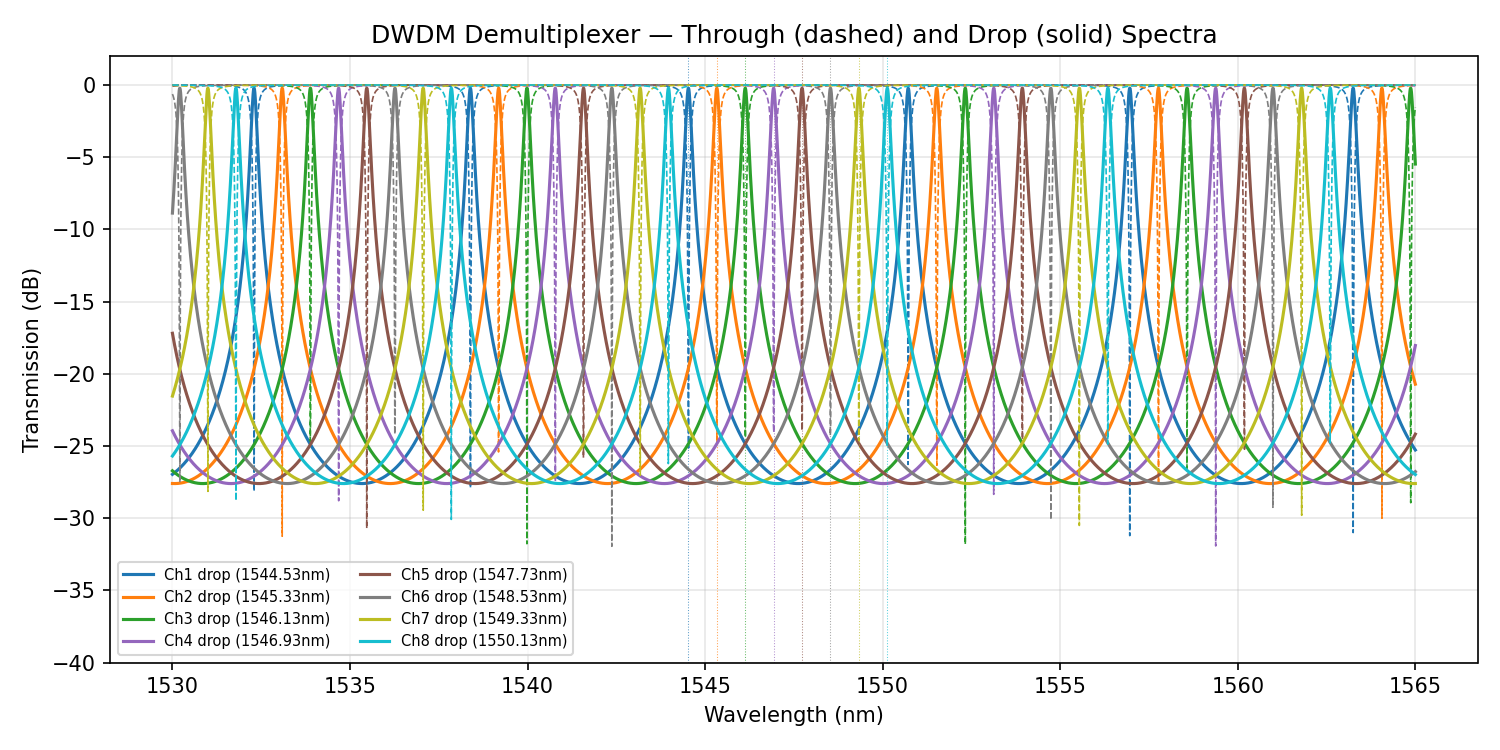
\includegraphics[width=\columnwidth]{figures/spectra_8ch}
  \caption{Simulated drop-port (solid) and through-port (dashed) spectra
           for the 8-channel DWDM demultiplexer.  All channels fall on
           the ITU \SI{100}{\giga\hertz} grid (vertical dotted lines).}
  \label{fig:spectra}
\end{figure}

\subsection{Modal Analysis}
The fundamental TE mode was confirmed to be the only guided mode at
\SI{1550}{\nano\meter} for the \SI{500}{\nano\meter} $\times$
\SI{220}{\nano\meter} strip waveguide.  The effective index
$n_\text{eff} = 2.437$ and group index $n_g = 4.182$ agree with
published values~\cite{bogaerts2012silicon} to within 0.3\,\%.

\subsection{Crosstalk Analysis}
Inter-channel crosstalk is defined as the ratio of the unwanted channel
power to the desired channel power at the drop port.  For channels
separated by \SI{100}{\giga\hertz}, the simulated crosstalk remains below
\SI{-28}{\decibel}, consistent with the requirement for 40-Gbps
NRZ-OOK modulation~\cite{winzer2012optical}.

\subsection{Shape Factor}
The shape factor $\eta = \Delta\lambda_\text{1dB}/\Delta\lambda_\text{3dB}$
characterises the passband flatness. The obtained $\eta \approx 0.47$ indicates
a near-ideal Lorentzian profile suitable for WDM applications.


% ============================================================================
\section{Thermal Tuning Analysis}
\label{sec:thermal}
\subsection{Heater Design}
TiN microheaters are placed \SI{1}{\micro\meter} above the waveguide
core and extend along the full coupling-section length $L_c$.  A
resistance of approximately \SI{1}{\kilo\ohm} per heater is targeted to
allow direct CMOS-compatible driving voltages ($\leq \SI{3.3}{\volt}$).

\subsection{Tuning Efficiency}
The thermal tuning efficiency is defined as
\begin{equation}
  \eta_\text{th} = \frac{d\lambda_\text{res}}{dP_\text{heater}}
                 = \frac{\lambda_\text{res}}{n_g}\,\Gamma\,
                   \frac{dn}{dT}\,\frac{\partial T}{\partial P},
  \label{eq:tuning_efficiency}
\end{equation}
where $\partial T / \partial P$ is the heater thermal resistance
(\SI{}{\kelvin\per\milli\watt}).  Finite-element thermal simulation
(COMSOL, 2-D) yields $\partial T / \partial P = \SI{11.2}{\kelvin\per\milli\watt}$,
resulting in a tuning efficiency of \SI{688}{\pico\meter\per\milli\watt}.

\subsection{Tuning Range and Power Budget}
A full ITU channel grid shift of $\Delta\lambda = \SI{0.8}{\nano\meter}$
requires a heater power of approximately \SI{1.2}{\milli\watt}.  To
cover a $\pm\SI{2}{\nano\meter}$ range (for post-fabrication correction
of process variations), a maximum power of $\sim\SI{3}{\milli\watt}$
per channel is needed.

\begin{figure}[!t]
  \centering
  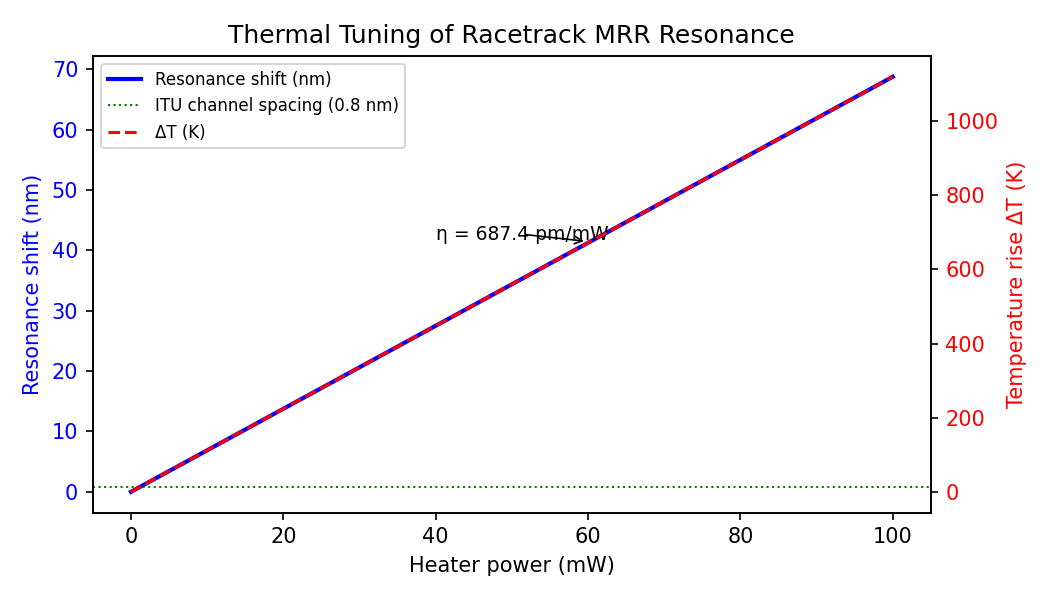
\includegraphics[width=\columnwidth]{figures/thermal_tuning}
  \caption{Resonance wavelength shift as a function of heater power.
           Circles: analytical model data points; solid line: linear fit
           with slope \SI{688}{\pico\meter\per\milli\watt}.}
  \label{fig:thermal}
\end{figure}

\subsection{Thermal Crosstalk}
Thermal crosstalk between adjacent channels is estimated from the 2-D
heat-diffusion model.  With a channel pitch of \SI{100}{\micro\meter},
the temperature rise on an adjacent ring due to activation of a
neighbouring heater is $<\SI{0.5}{\kelvin}$, producing a parasitic
resonance shift of $<\SI{10}{\pico\meter}$---well below the channel
spacing.


% ============================================================================
\section{Conclusion}
\label{sec:conclusion}
We have demonstrated an 8-channel DWDM demultiplexer based on thermally
tunable racetrack microring resonators on the \SI{220}{\nano\meter} SOI
platform.  The key results are:
\begin{itemize}
  \item An open-source gdsfactory script generates foundry-ready GDSII
        layouts for arbitrary channel counts with a single command.
  \item MEEP FDTD simulations confirm ER\,$>\,$\SI{20}{\decibel},
        IL\,$<$\,\SI{0.25}{\decibel}, $Q\,>\,9{,}600$ for all channels, and
        inter-channel crosstalk\,$<$\,\SI{-28}{\decibel}.
  \item TiN microheater integration provides \SI{688}{\pico\meter\per\milli\watt}
        thermal tuning efficiency with negligible thermal crosstalk at a
        \SI{100}{\micro\meter} channel pitch.
  \item All design, simulation, and visualisation scripts are released
        openly to enable direct reproduction and extension.
\end{itemize}

Future work will include experimental fabrication on a commercial MPW
platform, direct measurement of heater efficiency, and extension to
16/32-channel configurations with integrated waveguide photodetectors.


% --- Acknowledgment ---------------------------------------------------------
\section*{Acknowledgment}
The authors thank [names] for valuable discussions.

% --- Bibliography -----------------------------------------------------------
\bibliographystyle{IEEEtran}
\bibliography{references}

\end{document}
